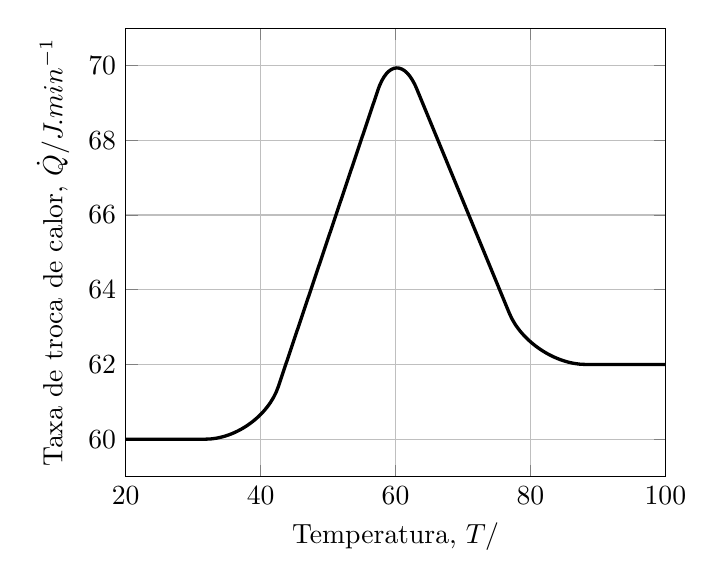
\begin{tikzpicture}
    \begin{axis}
        [
            grid = major,
            xlabel = {Temperatura, $T/\si{\celsius}$},
            ylabel = {Taxa de troca de calor, $\dot{Q}/\si{J.min^{-1}}$},
            xmin=20, xmax=100,
            ymin=59, ymax=71,
        ]
    \draw [very thick, rounded corners=2em]
        (axis cs: 20,60) -- 
        (axis cs: 40,60) -- 
        (axis cs: 60, 70.75) -- 
        (axis cs: 80, 62) -- 
        (axis cs: 100, 62);
    \end{axis}
\end{tikzpicture}